\section{Learning the reward}

\begin{frame}
    \frametitle{Learning the reward}

    Same as learning the optimality variable.

    \begin{align}
        p(\mathcal{O} | \mathbf{x}_t, \mathbf{u}_t, \psi) = exp(r_{\psi}(\mathbf{x}_t, \mathbf{u}_t)) \\
        p(\tau | \mathcal{O}, \psi) \propto p(\tau)\ exp(\sum_t r_{\psi}(\mathbf{x}_t, \mathbf{u}_t))
    \end{align}

    Note that $p(\tau)$ is not dependent on $\psi$.

    The whole thing becomes maximum likelihood learning:

    \begin{equation}
        \max_{\psi} \frac{1}{N} \sum_{i=1}^{N} log\ p(\tau_i | \mathcal{O}_{1:T}, \psi) = \max_{\psi} \frac{1}{N} \sum_{i=1}^{N} r_\psi (\tau_i) - log\ Z
    \end{equation}

\end{frame}

\begin{frame}
    \frametitle{Partition function}

    Normalizer (partition) function could be defined as:
    \begin{equation}
        Z = \int\ p(\tau)\ exp(r_\psi(\tau))\ d\tau
    \end{equation}

    Just compute gradient and optimize:

    \begin{equation}
        \nabla_\psi \mathcal{L} = \frac{1}{N} \sum_{i=1}^{N} \nabla_\psi\ r_\psi(\tau_i) - \frac{1}{Z} \int\ p(\tau)\ exp(r_\psi(\tau))\ \nabla_\psi\ r_\psi(\tau)\ d\tau
    \end{equation}

\end{frame}

\begin{frame}
    \frametitle{Partition function}

    But second term can be considered as expected value and equation becomes:

    % But second term is the expected value under the distribution of trajectories under psi

    \begin{equation}
        \nabla_\psi \mathcal{L}=E_{\tau \sim \pi^{\star}(\tau)}\left[\nabla_\psi r_\psi\left(\tau_i\right)\right]-E_{\tau \sim p\left(\tau \mid \mathcal{O}_{1: T}, \psi\right)}\left[\nabla_\psi r_\psi(\tau)\right]
    \end{equation}

    \begin{itemize}
        \item First item is estimation over expert samples
        \item Second item is soft optimal policy under current reward
    \end{itemize}
\end{frame}

\begin{frame}
    \frametitle{MaxEnt IRL algorithm \cite{ziebart_maximum_nodate}}

    \begin{itemize}
        \item compute probability of control given state being optimal for reward (backward message)
        \item compute probability of state begin optimal for reward (forward message)
        \item compute state-action visitation probability for pairs $(\mathbf{x}_t, \mathbf{u}_t)$
        \item evaluate gradient
        \item update
    \end{itemize}
\end{frame}

\begin{frame}
    \frametitle{Guided cost learning algorithm \cite{finn_guided_2016}}

    As summation over policy samples is quite costly, we can use weights:

    \begin{equation}
        w_j= \frac{p(\tau)\ exp(r_\psi(\tau_j))}{\pi(\tau_j)}
    \end{equation}

    \begin{center}
        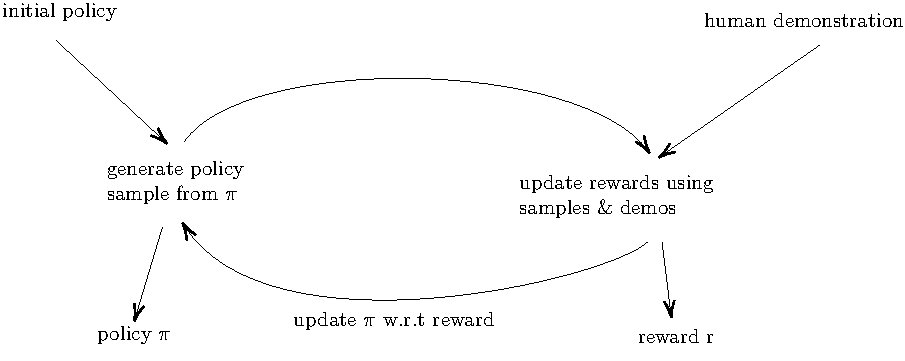
\includegraphics[width=0.7\linewidth]{content/tikz/guided_cost.pdf}
    \end{center}
\end{frame}